\documentclass[]{standalone}
\usepackage[T1]{fontenc}\usepackage{tikz}
\usepackage{amsmath, amsfonts}
\usepackage{xintexpr}
\usepackage{comment}
\usetikzlibrary{arrows, shapes.geometric, calc, positioning, decorations.pathreplacing}

\makeatletter
\def\input@path{{./includes/}{./includes/ut/diags/}}
\makeatother

\immediate\write18{zsh -c './27-practical-30-fig3-gen.py no_replace_recent entropy=1662350874' 2> 27-practical-30-fig3-autogen.log}

\begin{document}%
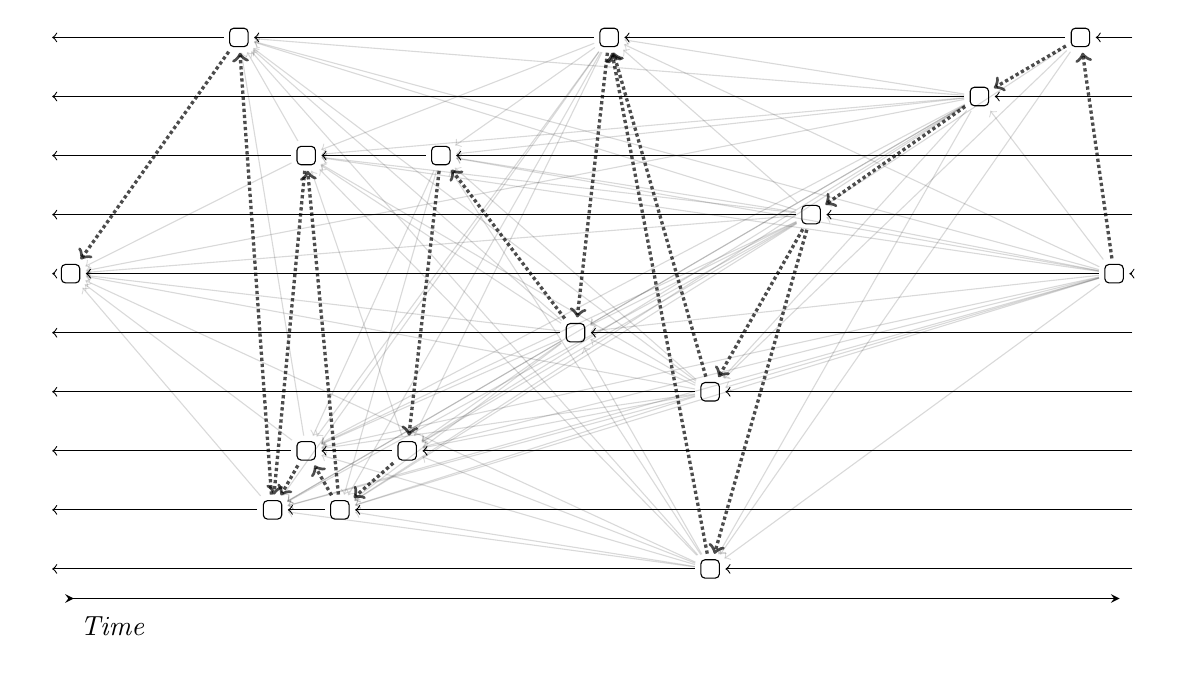
\begin{tikzpicture}[node distance=0.1cm]%
    \tikzstyle{block} = [draw, rounded corners=1.5pt, fill=white, fill opacity=0]

    \tikzstyle{ar} = [->, -to, shorten >= 2pt, shorten <= 2pt, opacity=0.6]

    \tikzstyle{arFocus} = [ar, densely dotted, very thick, opacity=0.7]
    \tikzstyle{arFocusTip} = [arFocus, color=red]
    \tikzstyle{arFocusOut} = [arFocus, color=blue]
    \tikzstyle{arFocusPrevTip} = [arFocus, color=red]
    \tikzstyle{arPreFocusOut} = [arFocus, color=blue]
    \tikzstyle{arFocusIn} = [arFocus, color=green]

    \tikzstyle{pAr} = [ar, opacity=1]
    \tikzstyle{arNone} = [ar, opacity=.15]

    \tikzstyle{arrowTime} = [stealth reversed-stealth, shorten >= -2pt, shorten <= -2pt]

    \def\scale{0.75cm}
    \edef\sx{2*0.285*\scale}
    \edef\sy{\scale}

    \def\timeArY{-0.5*\sy}
    \draw [arrowTime] (0, \timeArY) node () [anchor=west, yshift=-10pt] {\textit{Time}} -- (31*\sx, \timeArY);

    \node (c5t0) [block] at (0*\sx, 5*\sy) {};
\node (c5t-1) at (-1*\sx, 5*\sy) {};
\draw [pAr] (c5t0) -- (c5t-1);
\node (c9t5) [block] at (5*\sx, 9*\sy) {};
\node (c9t-1) at (-1*\sx, 9*\sy) {};
\draw [pAr] (c9t5) -- (c9t-1);
\draw [arFocus] (c9t5) -- (c5t0);
\node (c1t6) [block] at (6*\sx, 1*\sy) {};
\node (c1t-1) at (-1*\sx, 1*\sy) {};
\draw [pAr] (c1t6) -- (c1t-1);
\draw [arNone] (c1t6) -- (c5t0);
\draw [arFocus] (c1t6) -- (c9t5);
\node (c2t7) [block] at (7*\sx, 2*\sy) {};
\node (c2t-1) at (-1*\sx, 2*\sy) {};
\draw [pAr] (c2t7) -- (c2t-1);
\draw [arFocus] (c2t7) -- (c1t6);
\draw [arNone] (c2t7) -- (c5t0);
\draw [arNone] (c2t7) -- (c9t5);
\node (c7t7) [block] at (7*\sx, 7*\sy) {};
\node (c7t-1) at (-1*\sx, 7*\sy) {};
\draw [pAr] (c7t7) -- (c7t-1);
\draw [arFocus] (c7t7) -- (c1t6);
\draw [arNone] (c7t7) -- (c5t0);
\draw [arNone] (c7t7) -- (c9t5);
\node (c1t8) [block] at (8*\sx, 1*\sy) {};
\draw [pAr] (c1t8) -- (c1t6);
\draw [arFocus] (c1t8) -- (c2t7);
\draw [arFocus] (c1t8) -- (c7t7);
\node (c2t10) [block] at (10*\sx, 2*\sy) {};
\draw [pAr] (c2t10) -- (c2t7);
\draw [arFocus] (c2t10) -- (c1t8);
\draw [arNone] (c2t10) -- (c7t7);
\node (c7t11) [block] at (11*\sx, 7*\sy) {};
\draw [pAr] (c7t11) -- (c7t7);
\draw [arNone] (c7t11) -- (c1t8);
\draw [arFocus] (c7t11) -- (c2t10);
\draw [arNone] (c7t11) -- (c2t7);
\node (c4t15) [block] at (15*\sx, 4*\sy) {};
\node (c4t-1) at (-1*\sx, 4*\sy) {};
\draw [pAr] (c4t15) -- (c4t-1);
\draw [arNone] (c4t15) -- (c1t8);
\draw [arNone] (c4t15) -- (c1t6);
\draw [arNone] (c4t15) -- (c2t10);
\draw [arNone] (c4t15) -- (c2t7);
\draw [arNone] (c4t15) -- (c5t0);
\draw [arFocus] (c4t15) -- (c7t11);
\draw [arNone] (c4t15) -- (c7t7);
\draw [arNone] (c4t15) -- (c9t5);
\node (c9t16) [block] at (16*\sx, 9*\sy) {};
\draw [pAr] (c9t16) -- (c9t5);
\draw [arNone] (c9t16) -- (c1t8);
\draw [arNone] (c9t16) -- (c1t6);
\draw [arNone] (c9t16) -- (c2t10);
\draw [arNone] (c9t16) -- (c2t7);
\draw [arFocus] (c9t16) -- (c4t15);
\draw [arNone] (c9t16) -- (c7t11);
\draw [arNone] (c9t16) -- (c7t7);
\node (c0t19) [block] at (19*\sx, 0*\sy) {};
\node (c0t-1) at (-1*\sx, 0*\sy) {};
\draw [pAr] (c0t19) -- (c0t-1);
\draw [arNone] (c0t19) -- (c1t8);
\draw [arNone] (c0t19) -- (c1t6);
\draw [arNone] (c0t19) -- (c2t10);
\draw [arNone] (c0t19) -- (c2t7);
\draw [arNone] (c0t19) -- (c4t15);
\draw [arNone] (c0t19) -- (c5t0);
\draw [arNone] (c0t19) -- (c7t11);
\draw [arNone] (c0t19) -- (c7t7);
\draw [arFocus] (c0t19) -- (c9t16);
\draw [arNone] (c0t19) -- (c9t5);
\node (c3t19) [block] at (19*\sx, 3*\sy) {};
\node (c3t-1) at (-1*\sx, 3*\sy) {};
\draw [pAr] (c3t19) -- (c3t-1);
\draw [arNone] (c3t19) -- (c1t8);
\draw [arNone] (c3t19) -- (c1t6);
\draw [arNone] (c3t19) -- (c2t10);
\draw [arNone] (c3t19) -- (c2t7);
\draw [arNone] (c3t19) -- (c4t15);
\draw [arNone] (c3t19) -- (c5t0);
\draw [arNone] (c3t19) -- (c7t11);
\draw [arNone] (c3t19) -- (c7t7);
\draw [arFocus] (c3t19) -- (c9t16);
\draw [arNone] (c3t19) -- (c9t5);
\node (c6t22) [block] at (22*\sx, 6*\sy) {};
\node (c6t-1) at (-1*\sx, 6*\sy) {};
\draw [pAr] (c6t22) -- (c6t-1);
\draw [arFocus] (c6t22) -- (c0t19);
\draw [arNone] (c6t22) -- (c1t8);
\draw [arNone] (c6t22) -- (c1t6);
\draw [arNone] (c6t22) -- (c2t10);
\draw [arNone] (c6t22) -- (c2t7);
\draw [arFocus] (c6t22) -- (c3t19);
\draw [arNone] (c6t22) -- (c4t15);
\draw [arNone] (c6t22) -- (c5t0);
\draw [arNone] (c6t22) -- (c7t11);
\draw [arNone] (c6t22) -- (c7t7);
\draw [arNone] (c6t22) -- (c9t16);
\draw [arNone] (c6t22) -- (c9t5);
\node (c8t27) [block] at (27*\sx, 8*\sy) {};
\node (c8t-1) at (-1*\sx, 8*\sy) {};
\draw [pAr] (c8t27) -- (c8t-1);
\draw [arNone] (c8t27) -- (c0t19);
\draw [arNone] (c8t27) -- (c1t8);
\draw [arNone] (c8t27) -- (c1t6);
\draw [arNone] (c8t27) -- (c2t10);
\draw [arNone] (c8t27) -- (c2t7);
\draw [arNone] (c8t27) -- (c3t19);
\draw [arNone] (c8t27) -- (c4t15);
\draw [arNone] (c8t27) -- (c5t0);
\draw [arFocus] (c8t27) -- (c6t22);
\draw [arNone] (c8t27) -- (c7t11);
\draw [arNone] (c8t27) -- (c7t7);
\draw [arNone] (c8t27) -- (c9t16);
\draw [arNone] (c8t27) -- (c9t5);
\node (c9t30) [block] at (30*\sx, 9*\sy) {};
\draw [pAr] (c9t30) -- (c9t16);
\draw [arNone] (c9t30) -- (c0t19);
\draw [arNone] (c9t30) -- (c3t19);
\draw [arNone] (c9t30) -- (c6t22);
\draw [arFocus] (c9t30) -- (c8t27);
\node (c5t31) [block] at (31*\sx, 5*\sy) {};
\draw [pAr] (c5t31) -- (c5t0);
\draw [arNone] (c5t31) -- (c0t19);
\draw [arNone] (c5t31) -- (c1t8);
\draw [arNone] (c5t31) -- (c1t6);
\draw [arNone] (c5t31) -- (c2t10);
\draw [arNone] (c5t31) -- (c2t7);
\draw [arNone] (c5t31) -- (c3t19);
\draw [arNone] (c5t31) -- (c4t15);
\draw [arNone] (c5t31) -- (c6t22);
\draw [arNone] (c5t31) -- (c7t11);
\draw [arNone] (c5t31) -- (c7t7);
\draw [arNone] (c5t31) -- (c8t27);
\draw [arFocus] (c5t31) -- (c9t30);
\draw [arNone] (c5t31) -- (c9t16);
\draw [arNone] (c5t31) -- (c9t5);
\node (c0t32) at (32*\sx, 0*\sy) {};
\draw [pAr] (c0t32) -- (c0t19);
\node (c1t32) at (32*\sx, 1*\sy) {};
\draw [pAr] (c1t32) -- (c1t8);
\node (c2t32) at (32*\sx, 2*\sy) {};
\draw [pAr] (c2t32) -- (c2t10);
\node (c3t32) at (32*\sx, 3*\sy) {};
\draw [pAr] (c3t32) -- (c3t19);
\node (c4t32) at (32*\sx, 4*\sy) {};
\draw [pAr] (c4t32) -- (c4t15);
\node (c5t32) at (32*\sx, 5*\sy) {};
\draw [pAr] (c5t32) -- (c5t31);
\node (c6t32) at (32*\sx, 6*\sy) {};
\draw [pAr] (c6t32) -- (c6t22);
\node (c7t32) at (32*\sx, 7*\sy) {};
\draw [pAr] (c7t32) -- (c7t11);
\node (c8t32) at (32*\sx, 8*\sy) {};
\draw [pAr] (c8t32) -- (c8t27);
\node (c9t32) at (32*\sx, 9*\sy) {};
\draw [pAr] (c9t32) -- (c9t30);
\end{tikzpicture}%
\end{document}
